\documentclass{article}

\usepackage{postprocess/context/arxiv}

\usepackage[utf8]{inputenc} % allow utf-8 input
\usepackage[T1]{fontenc}    % use 8-bit T1 fonts
\usepackage{hyperref}       % hyperlinks
\usepackage{url}            % simple URL typesetting
\usepackage{booktabs}       % professional-quality tables
\usepackage{amsfonts}       % blackboard math symbols
\usepackage{nicefrac}       % compact symbols for 1/2, etc.
\usepackage{microtype}      % microtypography
\usepackage{lipsum}		% Can be removed after putting your text content
\usepackage{graphicx}
\usepackage{natbib}
\usepackage{doi}
\usepackage{float}
\usepackage{subcaption}

\title{Causal Discovery Report on Linear-gaussian\_id\_0\_data}

\author{ \href{https://orcid.org/0000-0000-0000-0000}{
\includegraphics[scale=0.06]{postprocess/context/orcid.pdf}\hspace{1mm}Causal Copilot}}

\renewcommand{\headeright}{Technical Report}
\renewcommand{\undertitle}{Technical Report}

\hypersetup{
pdftitle={Causal Discovery Report on Linear-gaussian\_id\_0\_data},
pdfauthor={Causal Copilot},
pdfkeywords={Causal Discovery, Large Language Model, PC},
}

\begin{document}
\maketitle

\begin{abstract}
This report presents a comprehensive causal discovery analysis on a dataset characterized by linear relationships and Gaussian noise, utilizing advanced statistical methods to elucidate underlying causal structures. We applied the PC, GES, and NOTEARS algorithms, selected through a systematic process assisted by a large language model (LLM), ensuring an informed choice based on the dataset's properties. The analysis revealed intricate interdependencies, particularly highlighting the causal relationships where X3 influences both X2 and X5, and a feedback loop exists between X3 and X5. While robust bootstrap probabilities support the presence of edges X3 $\rightarrow$ X5 and X5 $\rightarrow$ X3, the lack of confidence in edges X1 $\rightarrow$ X2 and X3 $\rightarrow$ X2 emphasizes the need for cautious interpretation of the results. Our findings contribute to the field of causal inference by demonstrating a structured methodology for causal discovery in data lacking prior knowledge, ultimately paving the way for future research and practical applications in understanding complex variable relationships.
\end{abstract}

\keywords{Causal Discovery, Large Language Model, PC}

\raggedbottom
\section{Introduction}
In the realm of data analysis, causal discovery plays a pivotal role in uncovering the underlying relationships and influences among variables within a dataset. This report aims to explore a dataset that lacks any prior knowledge, presenting a unique opportunity to apply causal inference techniques to identify potential causal structures. By leveraging advanced algorithms and statistical methods, we seek to elucidate the interdependencies among the variables, thereby providing insights that could inform future research, policy decisions, or practical applications. Through this process, we aim to not only enhance our understanding of the data but also contribute to the broader field of causal analysis, which holds significant implications across various domains.

\section{Dataset Descriptions and EDA}
The following is a preview of our original dataset.

\begin{table}[H]
    \centering
    \caption{Dataset Preview}
    \begin{tabular}{rrrrr}
\toprule
       X1 &        X2 &        X3 &        X4 &        X5 \\
\midrule
 0.759270 &  3.791941 &  1.275057 & -0.704150 & -2.355544 \\
 0.280090 & -0.286466 &  0.359843 & -0.584496 & -0.433161 \\
-0.762616 & -2.749523 & -0.717714 & -0.083012 &  1.138534 \\
 0.044478 &  2.934581 &  2.305376 &  1.769520 & -1.891772 \\
-1.197811 & -3.484751 &  1.217528 &  0.086088 & -2.117598 \\
\bottomrule
\end{tabular}

\end{table}

\subsection{Data Properties}
We employ several statistical methods to identify data properties.

The shape of the data, data types, and missing values are assessed directly from the dataframe. Linearity is evaluated using Ramsey’s RESET test, followed by the Benjamini \& Yekutieli procedure for multiple test correction. Gaussian noise is assessed through the Shapiro-Wilk test, also applying the Benjamini \& Yekutieli procedure for multiple test correction. Time-Series and Heterogeneity are derived from user queries.

Properties of the dataset we analyzed are listed below.

\begin{table}[H]
    \centering
    \caption{Data Properties}

    \begin{tabular}{rrrrrrr}
    \toprule
    Shape ($n$ x $d$) & Data Type & Missing Value & Linearity & Gaussian Errors & Time-Series & Heterogeneity \\
    \midrule
    (2500, 5)   & Continuous & False & True & True & False & False \\
    \bottomrule
    \end{tabular}
        
\end{table}

\subsection{Distribution Analysis}
The following figure shows distributions of different variables. The orange dash line represents the mean, and the black line represents the median. Variables are categorized into three types according to their distribution characteristics.

\begin{figure}[H]
\centering
\includegraphics[width=\linewidth]{test_data/20241025_225531_Linear-Gaussian_id_0_nodes5_samples2500/output_graph/eda_dist.jpg}
\caption{\label{fig:dist}Distribution Plots of Variables}
\end{figure}

\begin{itemize}
\item Slight left skew distributed variables: X2
\item Slight right skew distributed variables: X1, X3, X4, X5
\item Symmetric distributed variables: None
\end{itemize}

\subsection{Correlation Analysis}

\begin{minipage}[t]{0.5\linewidth}
    In this analysis, we will categorize the correlation statistics of features in the dataset into three distinct categories: Strong correlations ($r>0.8$), Moderate correlations ($0.5<r<0.8$), and Weak correlations ($r<0.5$).

\begin{itemize}
\item Strong Correlated Variables: None
\item Moderate Correlated Variables: X2 and X1, X3 and X2
\item Weak Correlated Variables: X5 and X3
\end{itemize}
\vfill
\end{minipage}
\hfill
\begin{minipage}[t]{0.5\linewidth}
    \begin{figure}[H]
        \centering
        \vspace{-1.5cm}
        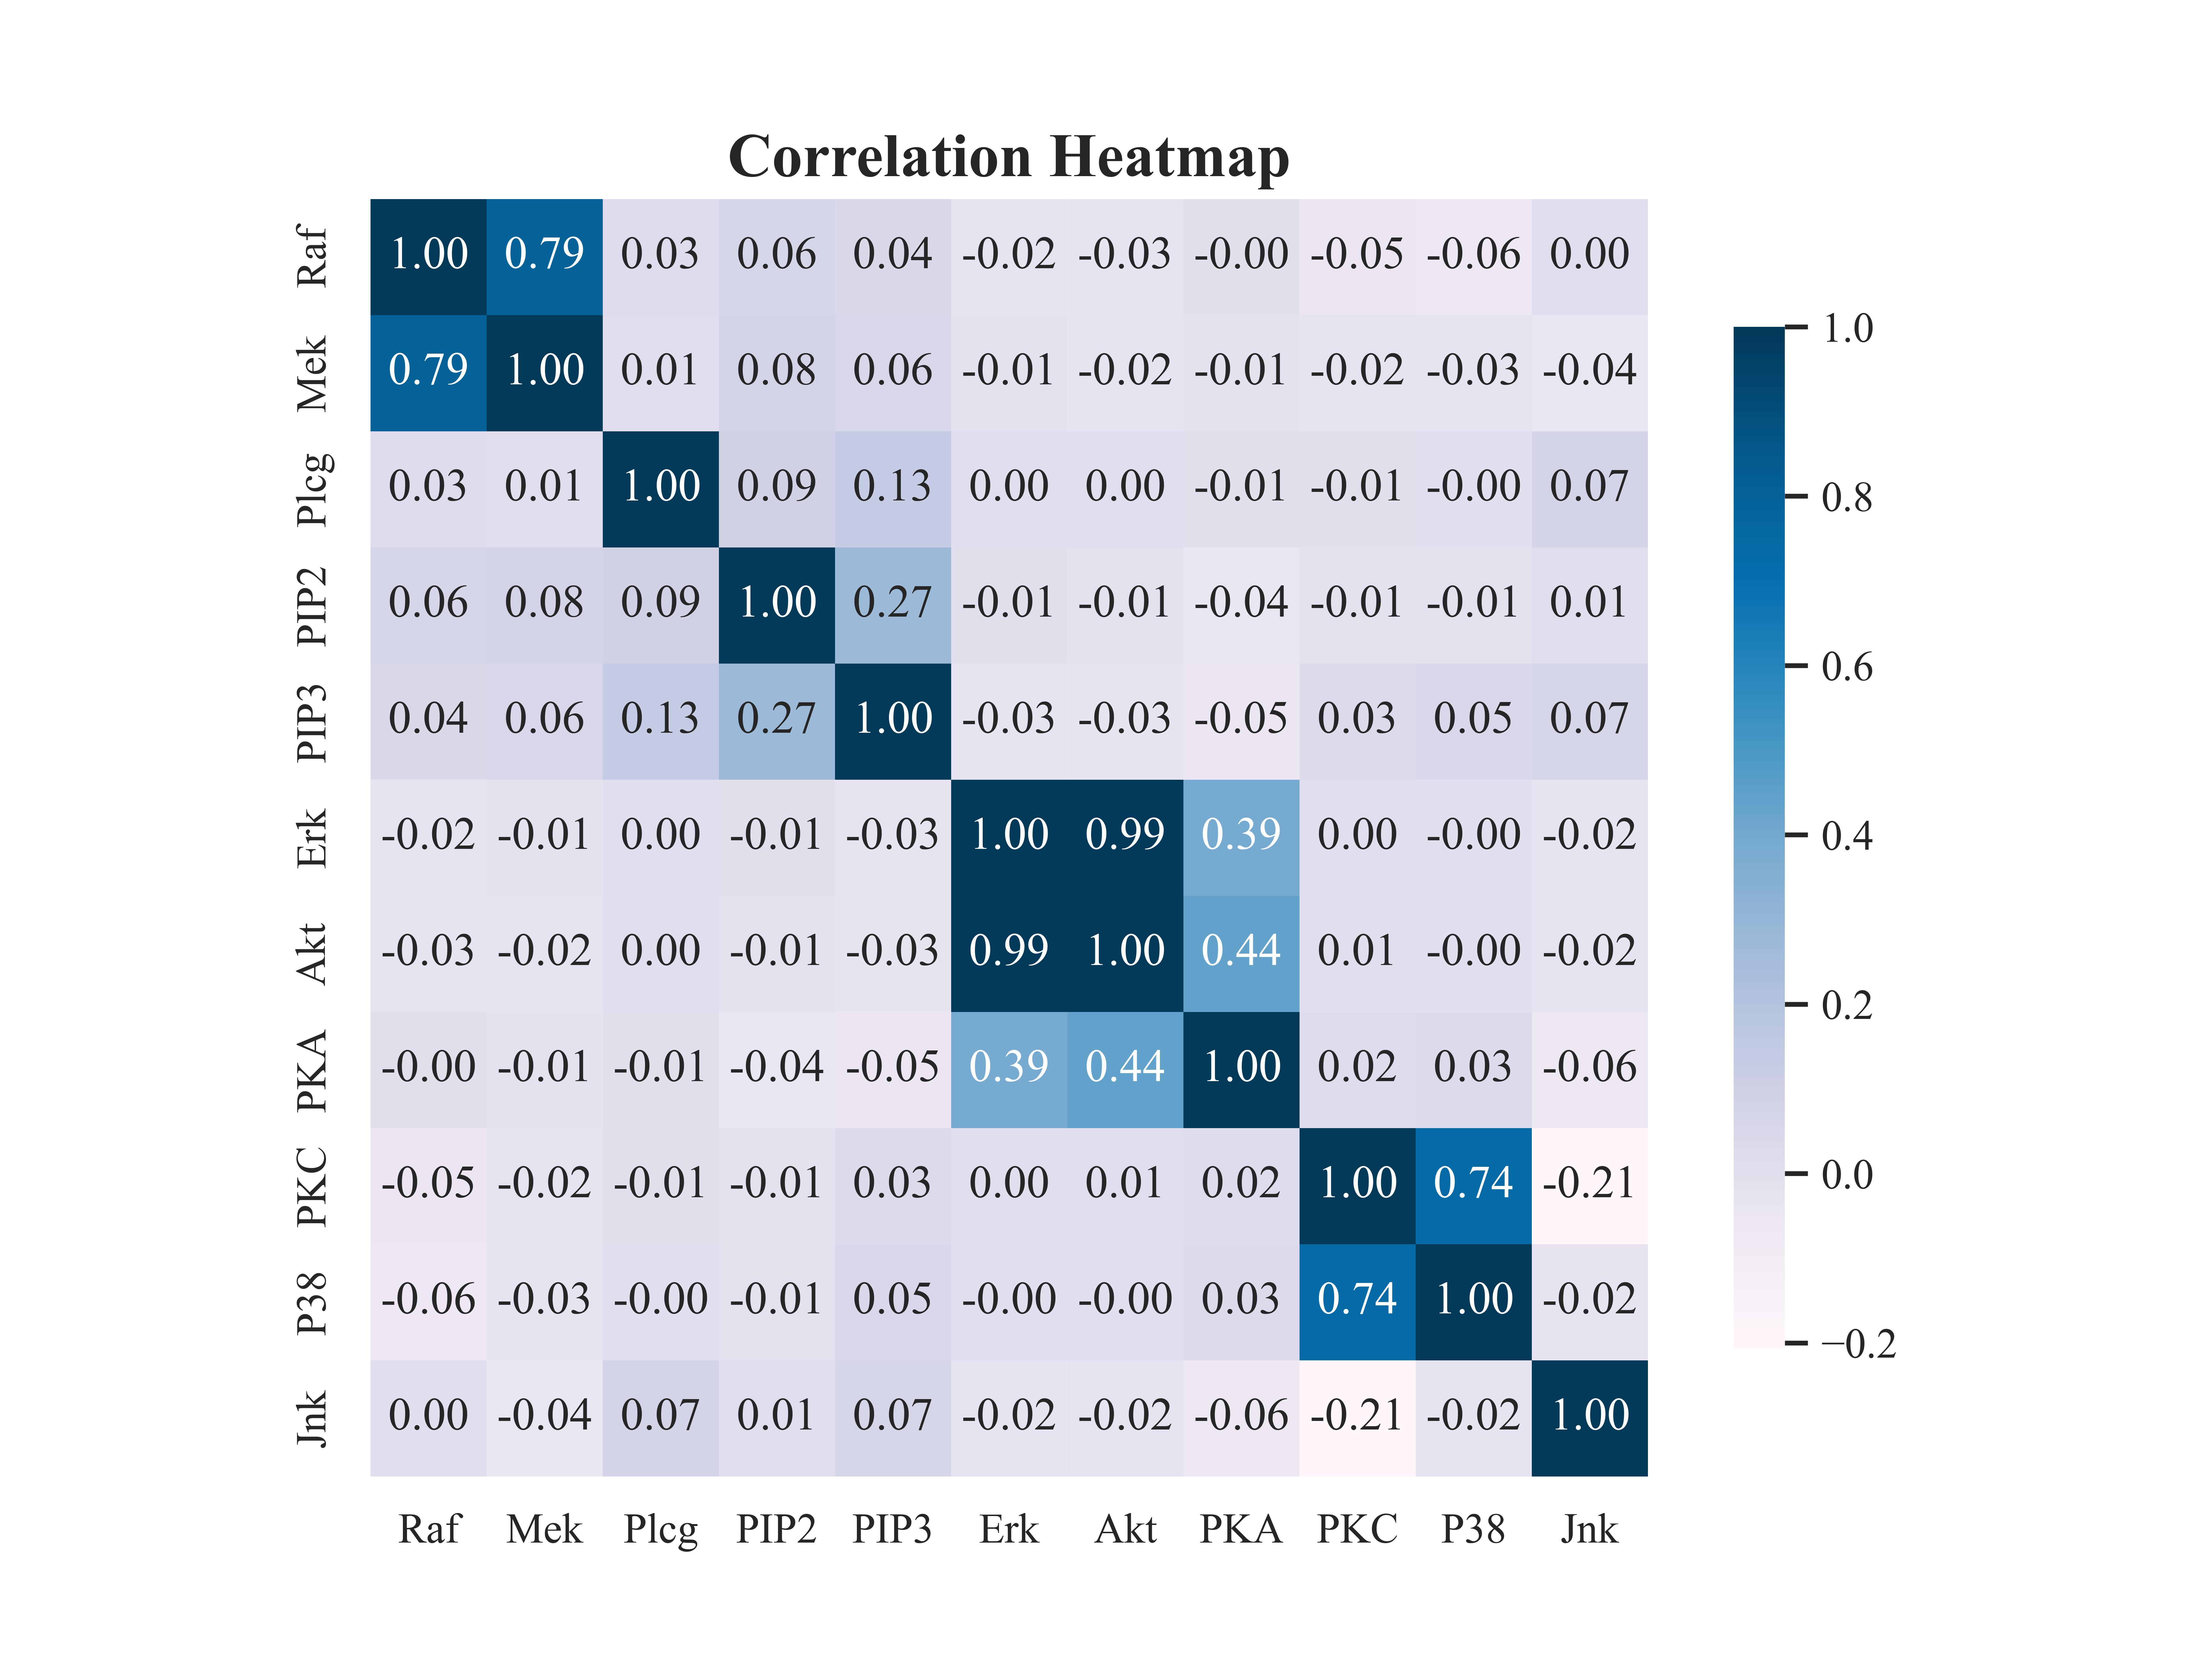
\includegraphics[width=\linewidth]{test_data/20241025_225531_Linear-Gaussian_id_0_nodes5_samples2500/output_graph/eda_corr.jpg}
        \caption{\label{fig:corr}Correlation Heatmap of Variables}
    \end{figure}
\end{minipage}

\section{Discovery Procedure}

In this section, we provide a detailed description of the causal discovery process implemented by Causal Copilot. We also provide the chosen algorithms and hyperparameters, along with the justifications for these selections.

\subsection{Data Preprocessing}
In this initial step, we preprocessed the data and examined its statistical characteristics. This involved cleaning the data, handling missing values, and performing exploratory data analysis to understand distributions and relationships between variables.
                
\subsection{Algorithm Selection assisted with LLM}
Following data preprocessing, we employed a large language model (LLM) to assist in selecting appropriate algorithms for causal discovery based on the statistical characteristics of the dataset and relevant background knowledge. The top three chosen algorithms, listed in order of suitability, are as follows:   
        
\begin{itemize}
    \item \textbf{PC}:
    \begin{itemize}
        \item \textbf{Description}: The PC algorithm is a constraint-based method that learns the structure of a causal graph from data by testing conditional independencies between variables. It constructs a directed acyclic graph (DAG) representing the causal relationships.
        \item \textbf{Justification}: Given the dataset's characteristics of linearity, Gaussian error distribution, and absence of hidden confounders, the PC algorithm is suitable for efficiently discovering causal relationships in large-scale datasets.
    \end{itemize}

    \item \textbf{GES}:
    \begin{itemize}
        \item \textbf{Description}: Greedy Equivalence Search (GES) identifies the optimal causal structure by navigating the space of equivalence classes of Directed Acyclic Graphs (DAGs) using a score function to evaluate and optimize the graph structure.
        \item \textbf{Justification}: The GES algorithm is effective for this dataset due to its large sample size, linear relationships, and Gaussian noise. It efficiently navigates complex causal structures, making it a strong candidate for accurate causal discovery.
    \end{itemize}

    \item \textbf{NOTEARS}:
    \begin{itemize}
        \item \textbf{Description}: NOTEARS transforms the problem of learning Directed Acyclic Graphs (DAGs) into a continuous optimization problem. It assumes linear relationships and Gaussian noise, aiming for efficient scaling to large datasets.
        \item \textbf{Justification}: Considering the dataset's linearity and relatively large sample size, NOTEARS offers a robust approach for learning the causal structure while effectively handling the linear relationships present in the data.
    \end{itemize}

\end{itemize}
                    

\subsection{Hyperparameter Values Proposal assisted with LLM}
Once the algorithms were selected, the LLM aided in proposing hyperparameters for the [ALGO] algorithm, which are specified below:
        
\begin{itemize}
    \item \textbf{alpha}:
    \begin{itemize}
        \item \textbf{Value}: 0.05
        \item \textbf{Explanation}: The sample size is significant (2500), allowing us to use a lower significance level to reduce false positives. An alpha of 0.05 is a standard choice for controlling Type I error rates in large samples.
    \end{itemize}

    \item \textbf{indep\_test}:
    \begin{itemize}
        \item \textbf{Value}: fisherz
        \item \textbf{Explanation}: Given that the dataset consists of continuous variables, the Fisher's Z test is the appropriate choice. It aligns well with the linear relationships and Gaussian errors present in the dataset.
    \end{itemize}

    \item \textbf{depth}:
    \begin{itemize}
        \item \textbf{Value}: -1
        \item \textbf{Explanation}: Setting depth to -1 allows the algorithm to consider all possible connections in the graph. This is preferable when the dataset's structure is unknown and all potential causal relations are to be explored.
    \end{itemize}
         
\end{itemize}

This structured approach ensures a comprehensive and methodical analysis of the causal relationships within the dataset.
        

\section{Results Summary}

\begin{figure}[H]
    \centering
    \begin{subfigure}{0.45\textwidth}
        \centering
        \vspace{-0.5cm}
        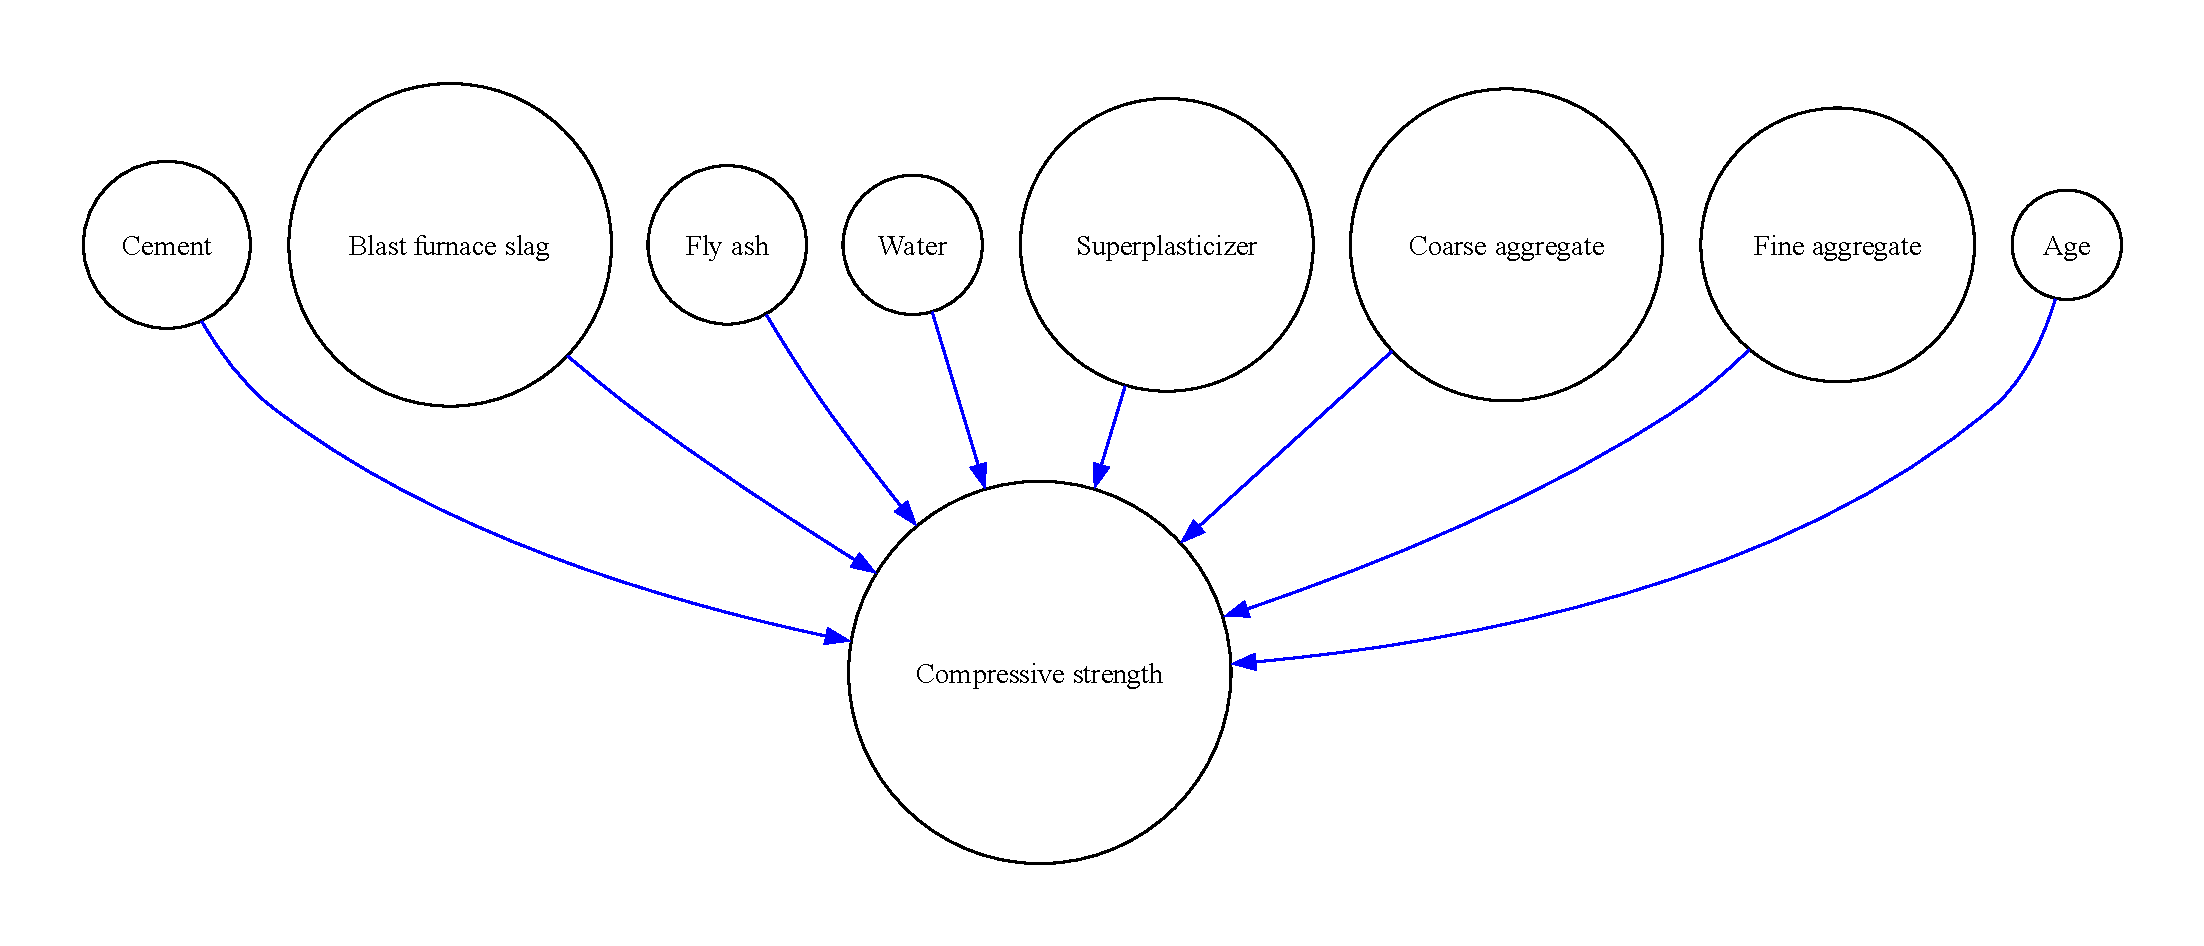
\includegraphics[width=\linewidth]{test_data/20241025_225531_Linear-Gaussian_id_0_nodes5_samples2500/output_graph/true_graph.pdf}
        \vfill
        \caption{True Graph}
        \label{fig:sub1}
    \end{subfigure}
    \hspace{0.04\textwidth}
    \begin{subfigure}{0.45\textwidth}
        \centering
        \vspace{-0.5cm}
        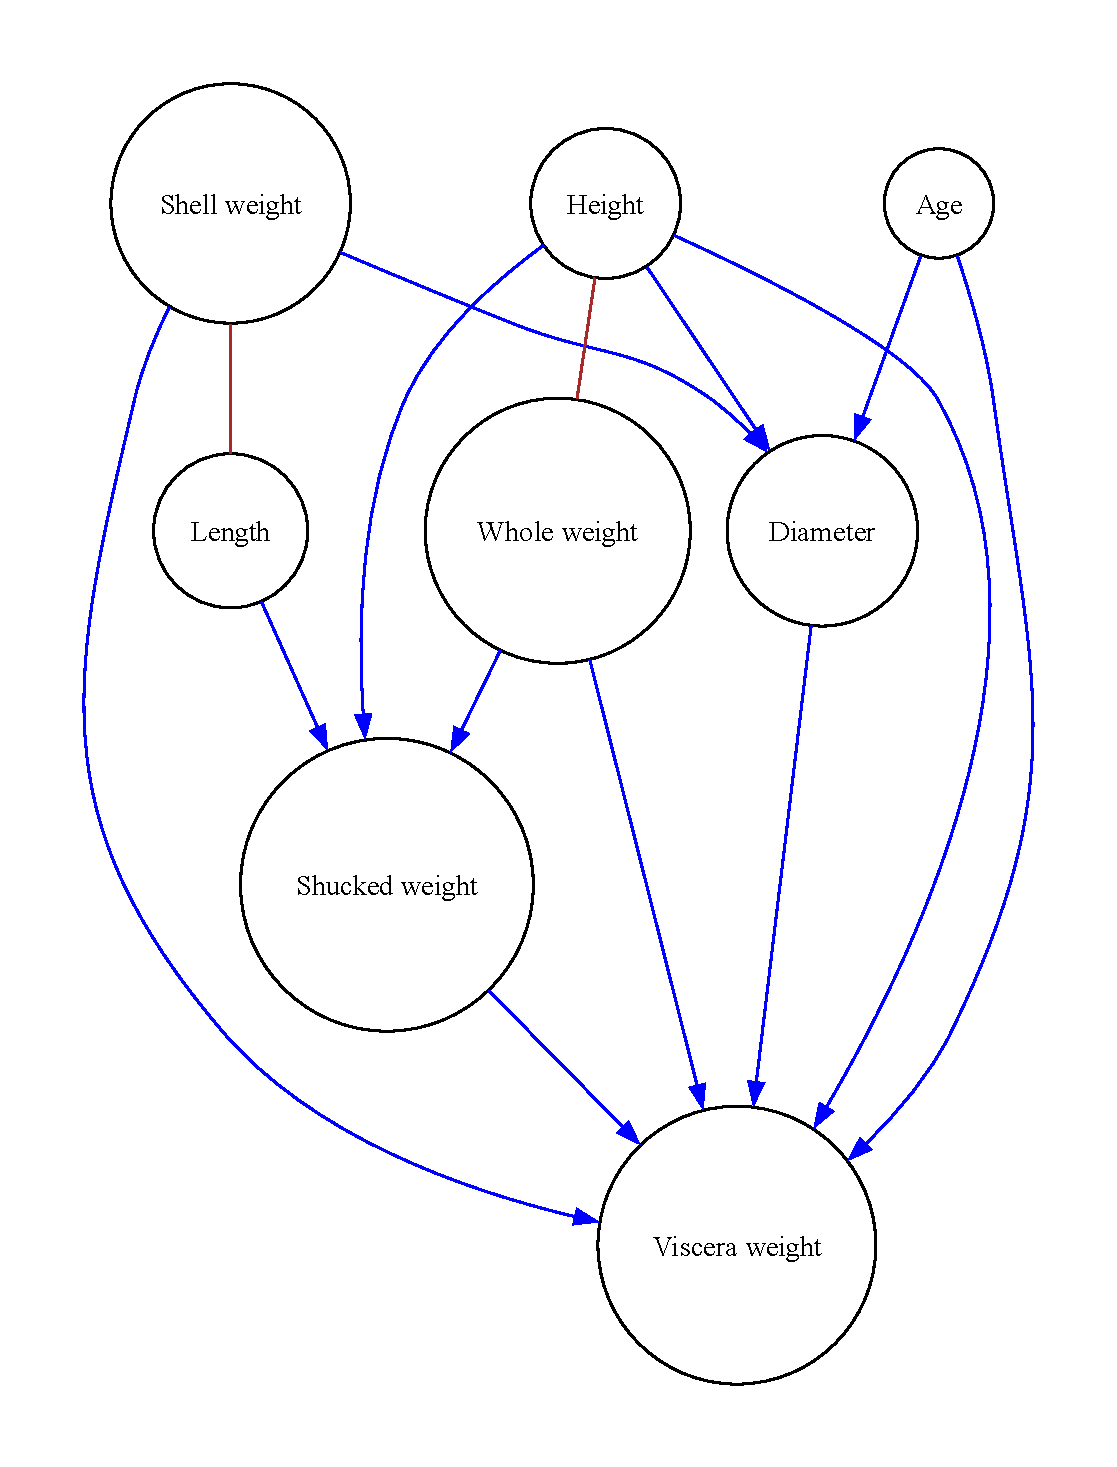
\includegraphics[width=\linewidth]{test_data/20241025_225531_Linear-Gaussian_id_0_nodes5_samples2500/output_graph/initial_graph.pdf}
        \vfill
        \caption{Initial Graph}
        \label{fig:sub2}
    \end{subfigure}
    \caption{Graphs Comparison of PC}
    \label{fig:main}
\end{figure}

The above are the true graph and the result graph produced by our algorithm.

The causal relationships among the variables reveal an intricate interplay where X2 is influenced by both X1 and X3, indicating that changes in X3 have a direct effect on X2 while also being a potential mediator for the impact of X1. Additionally, X3 exerts a significant causal influence over X5, suggesting that variations in X3 directly lead to changes in X5. Interestingly, there is also a feedback loop between X3 and X5, where X5 influences X3 in return, indicating a bidirectional relationship that may result in complex dynamics between these two variables. Overall, the relationships imply that while X1, X2, and X3 form a linear chain, X5 adds depth through its interaction with both X3 and potentially impacting X2 indirectly, hinting at a multifaceted causal structure among these variables.

\subsection{Graph Reliability Analysis}

\begin{figure}[H]
        \centering
        \vspace{-0.5cm}
        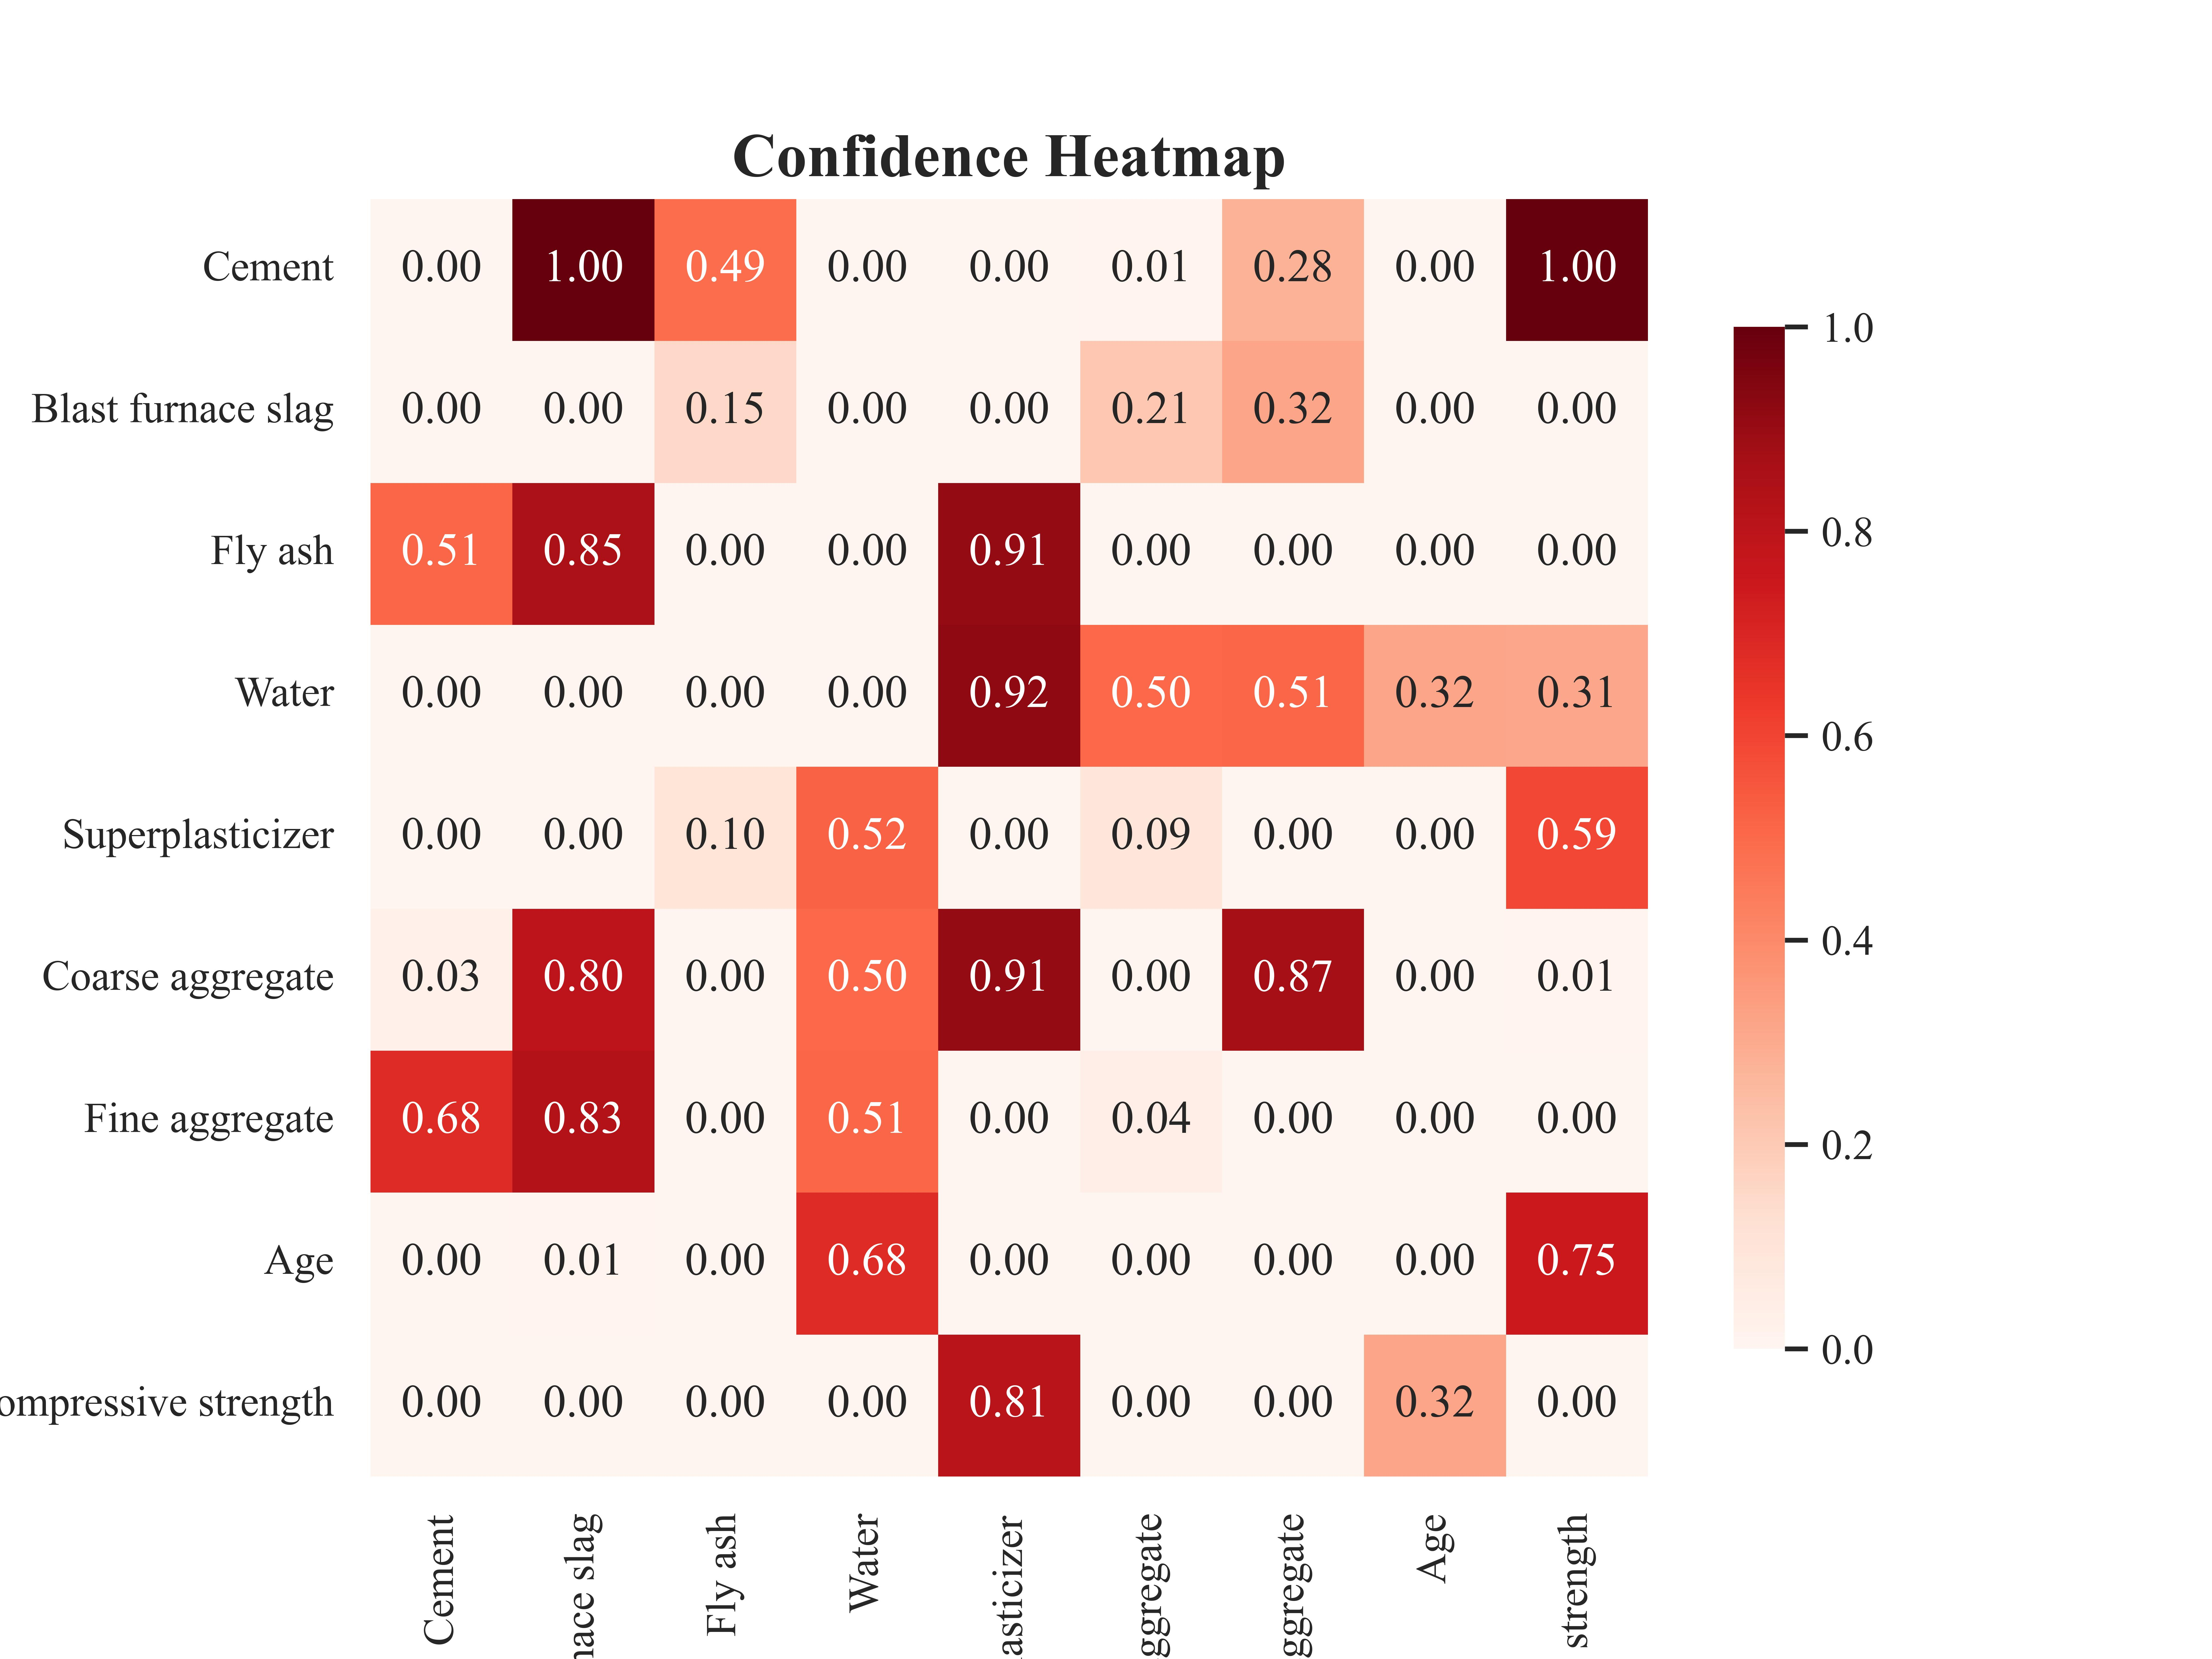
\includegraphics[width=0.8\linewidth]{test_data/20241025_225531_Linear-Gaussian_id_0_nodes5_samples2500/output_graph/confidence_heatmap.jpg}
        \caption{Reliability Graph}
        \label{fig:sub3}
\end{figure}

Based on the confidence probability heatmap and background knowledge, we can analyze the reliability of our graph.

From a statistical perspective, we have high confidence to believe that the edge X3 $\rightarrow$ X5 exists, as it has a bootstrap probability of 0.88, indicating substantial support for this causal relation. Additionally, the edge X5 $\rightarrow$ X3 is also highly reliable, with a bootstrap probability of 0.99, suggesting a strong reciprocal relationship between X3 and X5. However, we have low confidence in the edges X1 $\rightarrow$ X2 and X3 $\rightarrow$ X2, both having a bootstrap probability of 0.0, indicating no support for these causal relationships.

However, based on the expert knowledge, we have no additional information to suggest the existence of any edges, since the background knowledge noted is "No Knowledge." This lack of external validation means we cannot confirm or disconfirm any of the proposed edges beyond the statistical findings provided.

Therefore, considering both the bootstrap probabilities and the absence of expert knowledge, the result of this causal graph is not entirely reliable, especially with the nonsignificant edges indicating that we cannot confidently assert the validity of certain relationships within this causal framework.

\end{document}